\appendix
\chapter{Landau-Zener公式の証明}

\begin{equation}
  H = 
  \begin{pmatrix}
    -\frac{vt}{2} & \Delta_0\\
    \Delta_0 & \frac{vt}{2}
  \end{pmatrix}
\end{equation}
とする.また,系の状態ベクトルは,
\begin{equation}
  |\psi(t) \rangle = C_1(t) |1\rangle + C_2(t) |2\rangle
\end{equation}
である.さらに,系の初期状態は,$C_1(-\infty) = 1, C_2(-\infty) =0$としておく.このとき,Shr\"{o}dinger方程式より,
\begin{align}
  i\frac{d}{dt} C_1(t) &= -\frac{vt}{2} C_1(t) + \Delta_0 C_2(t) \label{LZ1}\\
  i\frac{d}{dt} C_2(t) &= \Delta_0 C_1(t) + \frac{vt}{2} C_2(t) \label{LZ2}\\
\end{align}
となる.式(\ref{LZ1})を微分して式(\ref{LZ2})を代入すると,
\begin{align}
  i\frac{d^2}{dt^2} C_1
  &= -\frac{v}{2} C_1(t) -\frac{vt}{2} C_1^{\prime} + \Delta_0 C_2^{\prime}\\
  &= -\frac{v}{2} C_1(t) -\frac{vt}{2} C_1^{\prime} + \Delta_0 \left( \frac{\Delta_0}{i} C_1 + \frac{vt}{2i} C_2 \right) \label{C1_A}
\end{align}
また,式(\ref{LZ2})を微分して式(\ref{LZ1})を代入すると.同様の計算から,
\begin{align}
 i\frac{d^2}{dt^2} C_2 = \frac{v}{2} C_2 + \frac{vt}{2} C_2^{\prime} + \Delta_0 \left( \frac{\Delta_0}{i} C_2 - \frac{vt}{2i} C_1 \right) \label{C2_A}
\end{align}
が得られる.したがって,式(\ref{C1_A})および式(\ref{C2_A})を整理すると,
\begin{align}
  \frac{d^2 C_1}{dt^2} + \left( \Delta_0^2 - \frac{iv}{2} \right) C_1 + \frac{v^2 t^2}{4} C_1 = 0\\
  \frac{d^2 C_2}{dt^2} + \left( \Delta_0^2 + \frac{iv}{2} \right) C_2 + \frac{v^2 t^2}{4} C_2 = 0\\
\end{align}
という$C_1$と$C_2$について独立な2つの方程式が得られる.ここで,
\begin{align}
  z &= i\sqrt{v} e^{i\frac{\pi}{4}} t \label{z_def}\\
  n &= i\delta\\
  \delta &= \frac{\Delta_0^2}{v}\\
  C_1 &= w_1(z)\\
  C_2 &= w_2(z)
\end{align}
という変数変換を行うと,
\begin{align}
  \frac{d^2 w_1}{d z^2} + \left(n + \frac{1}{2} - \frac{z^2}{4}\right) w_1 = 0\\
  \frac{d^2 C_2}{d z^2} + \left(n - \frac{1}{2} - \frac{z^2}{4}\right) w_2 = 0
\end{align}
が得られる.これらはWeberの微分方程式である.ここで,Weberの微分方程式の基本解である放物柱関数$D_n(z)$を用いて,
\begin{align}
  w_1 &\propto D_n(z)\\
  w_2 &\propto D_{n-1}(z)
\end{align}
としてよい.なぜなら,式(\ref{z_def})より,$t<0$で,
\begin{equation}
  z = i\sqrt{v} e^{i\frac{\pi}{4}} |t| = \sqrt{v} e^{-i\frac{\pi}{4}} |t|
\end{equation}
より,
\begin{equation}
  |\arg z| = \frac{\pi}{4} < \frac{3\pi}{4}
\end{equation}
であるから,放物柱関数$D_n(z)$に成り立つ定理
\begin{quote}
  $|z| \gg 1$のとき,$|\arg z| < \frac{3\pi}{4}$ならば
  \begin{equation}
    D_n(z) \rightarrow e^{-\frac{z^2}{4}} z^n
  \end{equation}
\end{quote}
を用いることができる.したがって,$t \rightarrow - \infty$で,
\begin{align}
  D_n(z) &= e^{-\frac{z^2}{4}} z^n\\
  D_{n-1}(z) &= e^{-\frac{z^2}{4}} z^{n-1}
\end{align}
と書ける.ここで,
\begin{align}
  z^n
  &= z^{i\delta}\\
  &= \exp(i\delta \log z)\\
  &= \exp(i\delta (\log \sqrt{v} e^{-\frac{i\pi}{4}} |t|))\\
  &= \exp \left( i\delta (\log (\sqrt{v} |t|) - \frac{i\pi}{4} \right)
\end{align}
より,$x \in \mathbb{R}$のとき,
\begin{align}
  D_n(z) = \exp \left( i\delta (\log (\sqrt{v} |t|) + \frac{\pi \delta}{4} \right) \label{D_n}\\
  D_{n-1}(z) = \frac{\exp \left( i\delta (\log (\sqrt{v} |t|) + \frac{\pi \delta}{4} \right)}{\sqrt{v} e^{-\frac{i\pi}{4}} |t|} \label{D_n-1}
\end{align}
であるから,$t \rightarrow -\infty$で,
\begin{align}
  |D_n(z)| &\rightarrow \text{有限}\\
  |D_{n-1}(z)| &\rightarrow 0
\end{align}
となる.これは,系の初期条件
\begin{align}
  C_1(-\infty) \ne 0\\
  C_2(-\infty) = 0
\end{align}
を満たす.したがって,任意定数$A,B$を用いて,
\begin{align}
  C_1(t) &= w_1(z) = A D_n(z),\\
  C_2(t) &= w_2(z) = B D_{n-1}(z)
\end{align}
としてよい.したがって,式(\ref{D_n})および式(\ref{D_n-1})より,$t \rightarrow -\infty$のとき,
\begin{align}
  \lim_{t \rightarrow -\infty} C_1(t) &= A \exp \left( \frac{ivt^2}{4} + \frac{\pi \delta}{4} + i\delta \log \sqrt{v} |t| \right) \label{C1_inf}\\
  \lim_{t \rightarrow -\infty} C_2(t) &= 0
\end{align}
である.


一方,$t \rightarrow \infty$のとき,
\begin{align}
  z &= \sqrt{v} e^{i\frac{3\pi}{4}},\\
  z^n
  &= z^{i\delta}\\
  &= \exp(i\delta \log z)\\
  &= \exp ( i\delta \log (\sqrt{v} t e^{i\frac{3\pi}{4}}))\\
  &= \exp \left( i\delta (\log \sqrt{v} t) + i\frac{3\pi}{4} \right)
\end{align}
となる.ここで,放物柱関数$D_n(z)$に成り立つ定理
\begin{quote}
  $\frac{\pi}{4} < \arg z < \frac{3\pi}{4}$のとき,
  \begin{equation}
    D_n(z) \rightarrow e^{-\frac{z^2}{4}} z^n - \frac{\sqrt{2\pi}}{\Gamma(-n)} e^{in\pi} e^{\frac{z^2}{4}} z^{-n-1}
  \end{equation}
\end{quote}
を用いる.このとき,$C_1(t)$については,$t \rightarrow \infty$で(第2項)$\rightarrow 0$より,
\begin{equation}
  \lim_{t\rightarrow \infty} C_1(t) = A \exp \left( \frac{ivt^2}{4} - \frac{e\pi \delta}{4} + i\delta \log (\sqrt{v}t) \right) \label{C1_lim2}
\end{equation}
となる.また,$C_2(t)$については,$t \rightarrow \infty$(第1項)$\rightarrow 0$より,
\begin{align}
  \lim_{t \rightarrow \infty} C_2(t)
  &= -B \frac{\sqrt{2 \pi}}{\Gamma(n+1)} e^{i(n-1) \pi} e^{\frac{z^2}{4}} z^{-n} \\
  &= -B \frac{\sqrt{2 \pi}}{\Gamma(1-i \delta)} \exp \left(i(i \delta-1) \pi-\frac{i v t^2}{4}-i \delta \log (\sqrt{v} t) \frac{3 \pi   \delta}{4}\right) \\
  & = B \frac{\sqrt{2 \pi}}{\Gamma(1-i \delta)} \exp \left(-\frac{\pi \delta}{4}-\frac{i v t^2}{4}-i \delta \log \sqrt{v} t\right)
\end{align}
となる.したがって,式(\ref{C1_inf})および式(\ref{C1_lim2})より,
\begin{equation}
  \frac{\lim_{t \rightarrow \infty} C_1(t)}{\lim_{t \rightarrow -\infty} C_1(t)} = \exp (-\pi \delta)
\end{equation}
であり,Landau-Zener公式
\begin{equation}
  P = \left| \frac{\lim_{t \rightarrow \infty} C_1(t)}{\lim_{t \rightarrow -\infty} C_1(t)} \right|^2  = \exp(-2\pi \delta)
\end{equation}
が示された.

\chapter{Dykhne-Davis-Pechukas法}
Shr\"{o}dinger方程式
\begin{equation}
  i\hbar \frac{d}{dt} |\psi(t) \rangle = H(t) |\psi(t) \rangle
\end{equation}
で,
\begin{align}
  |\psi(t) \rangle = a_1(t) \exp \left(-i \int_0^t d\tau \frac{E_1(\tau)}{\hbar} \right) |\phi_1(t)\rangle + a_2(t) \exp \left(-i \int_0^t d\tau \frac{E_2(\tau)}{\hbar} \right) |\phi_2(t)\rangle
\end{align}
を仮定する.ただし,$|\phi_i(t)\rangle$は断熱状態である.このとき,
\begin{align}
  a_1^{\prime} &= -\gamma \exp \left( -\frac{i\Delta}{\hbar} \right) a_2\\
  a_2^{\prime} &= \gamma \exp \left( \frac{i\Delta}{\hbar} \right) a_1
\end{align}
となる.ただし,
\begin{align}
  \gamma(t) &:= \langle \phi_1 | \phi_2^{\prime} \rangle\\
  \Delta(t) &:= \int_0^t d\tau (E_2 - E_1)
\end{align}
を定義した.ここで,$\Delta(t_c) = 0$となる$\Delta(t)$の零点$t_c$を用いて,
\begin{align}
  \tilde{a}_1 &= a_1(t)\\
  \tilde{a}_2 &= \exp \left( - \frac{i\Delta_c}{\hbar} \right) a_2(t)
\end{align}
を定義する.このとき,
\begin{align}
  \tilde{a}_1^{\prime} &= -\gamma \exp \left( \frac{-i (\Delta - \Delta_c)}{\hbar} \right) \tilde{a}_1\\
  \tilde{a}_2^{\prime} &= \gamma \exp \left( \frac{i (\Delta - \Delta_c)}{\hbar} \right) \tilde{a}_2
\end{align}
が成り立つ.ここで,図\ref{fig:Integral_path}のような複素積分区間を考える.また,$a_1(t_+)$および$a_2(t_+)$は,$a_1(t_-)$および$a_2(t_-)$から求められる.すなわち,
\begin{align}
  \begin{pmatrix}
    a_1(t_+)\\
    a_2(t_+)
  \end{pmatrix}
  =
  \begin{pmatrix}
    1_- & \Gamma_-\\
    \Gamma_+ & 1_+
  \end{pmatrix}
  \begin{pmatrix}
    a_1(t_-)\\
    a_2(t_-)
  \end{pmatrix} \label{Appendix_TM}
\end{align}
と書ける.ただし,
\begin{equation}
  \exp (\pm) := \exp \left(\pm \frac{i (\Delta - \Delta_c)}{\hbar}\right)
\end{equation}
とする.また,
\begin{align}
  1_{\pm} &= 1 - \int_{t_-}^{t_+} dt_1 \gamma \exp(\pm) \int_{t_-}^{t_1} dt_2 \gamma \exp(\mp)\\
  \Gamma_{\pm} &= \pm \int_{t_-}^{t_+} dt_1 \gamma \exp(\mp) - \int_{t_-}^{t_+} dt_1 \gamma \exp(\pm) \int_{t_-}^{t_1} dt_2 \gamma \exp(\mp) \int_{t_-}^{t_2} dt_3 \gamma \exp(\pm)
\end{align}
とする.式(\ref{Appendix_TM})に含まれる転送行列は,$\hbar \rightarrow 0$のとき,
\begin{equation}
  \begin{pmatrix}
    1_- & \Gamma_-\\
    \Gamma_+ & 1_+
  \end{pmatrix}
  \rightarrow
  \begin{pmatrix}
    1 & 0\\
    1 & 1
  \end{pmatrix}
\end{equation}
であることが知られている\cite{DavisPechukas1976}.


\begin{figure}[htbp]
  \centering
  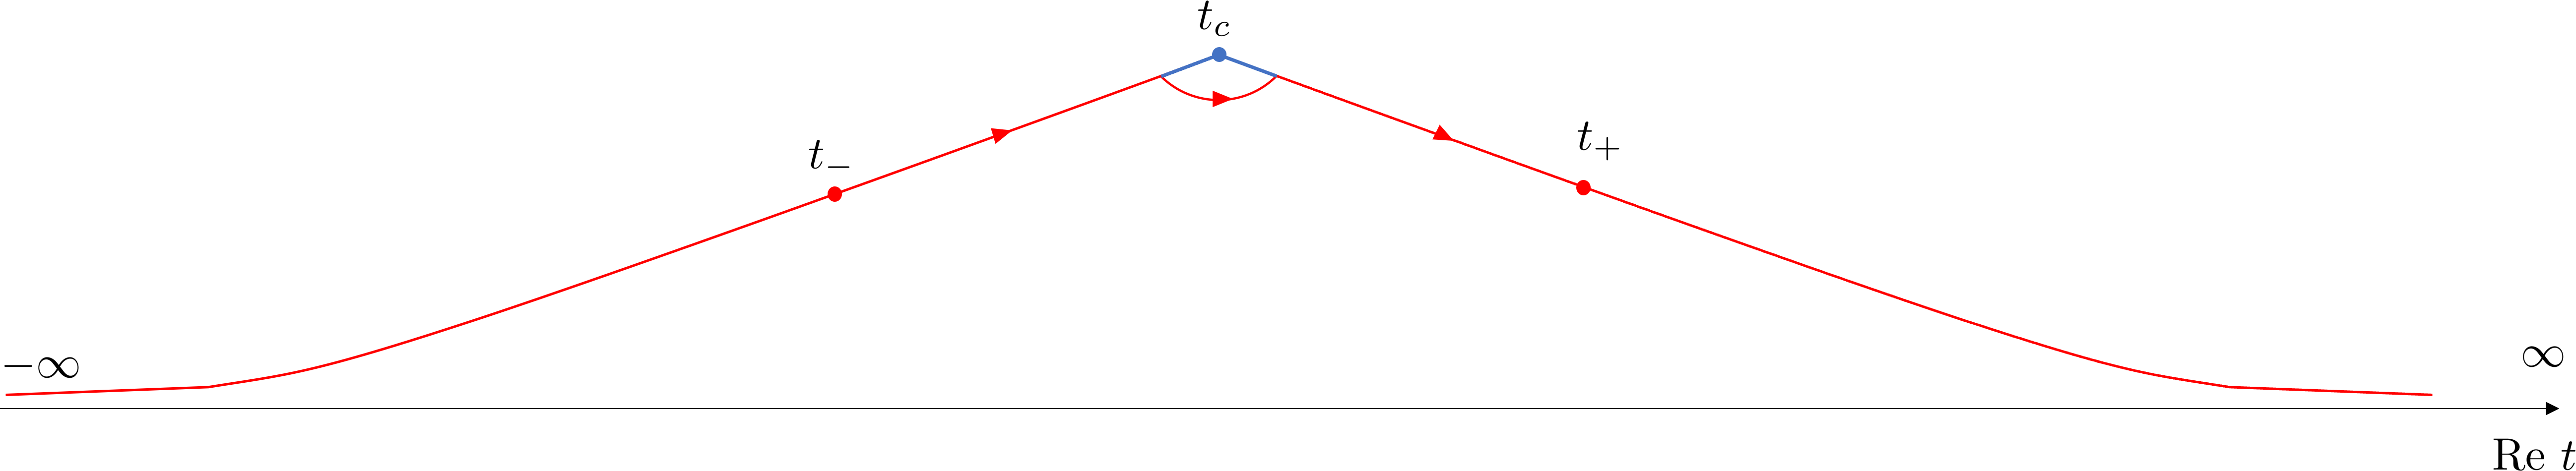
\includegraphics[scale=0.35]{figures/Integral_path.png}
  \caption{付録Bにおける複素積分の積分区間.$t_-$から$t_c$までの経路および$t_c$から$t_+$までの経路は"arm"あるいは"tail"と呼ぶ.また,$t_c$を迂回するような扇形の経路は,"center contour"と呼ぶ.}
  \label{fig:Integral_path}
\end{figure}


ここでは,特に重要な$\Gamma_+ \rightarrow 1$のみを示そう.任意の実対称Hamiltonian
\begin{equation}
  H =
  \begin{pmatrix}
    H_{11} & H_{12}\\
    H_{21} & H_{22}
  \end{pmatrix}
\end{equation}
の固有値は,
\begin{align}
  E_{\pm}
  &= \frac{H_{11} + H_{22}}{2} \pm \frac{\sqrt{(H_{11}-H_{22})^2 + 4 H_{12}^2}}{2}\\
  &:= \bar{E} \pm \frac{\delta E}{2}
\end{align}
となる.また,
\begin{align}
  H &= \bar{E} + \frac{\delta E}{2} 
  \begin{pmatrix}
    -\cos\theta & \sin \theta\\
    \sin\theta & \cos\theta
  \end{pmatrix}\\
  \tan \theta &= -\frac{2H_{12}}{H_{11}-H_{22}} \label{tan}\\
  \exp(2i\theta) &= \frac{H_{11} - H_{22} - 2i H_{12}}{H_{11} - H_{22} + 2i H_{12}} \label{exp}
\end{align}
と書ける\footnote{式(\ref{tan})と式(\ref{exp})は等価である.}.このとき,固有ベクトルは,
\begin{align}
  |\phi_1\rangle &= 
  \begin{pmatrix}
    \cos \frac{\theta}{2}\\
    -\sin \frac{\theta}{2}
  \end{pmatrix}\\
  |\phi_2\rangle &= 
  \begin{pmatrix}
    \sin \frac{\theta}{2}\\
    \cos \frac{\theta}{2}
  \end{pmatrix}\\  
\end{align}
となる.したがって,nonadiabatic coupling $\gamma$は
\begin{equation}
  \gamma = \pm \frac{\theta^{\prime}}{2} \label{gamma_B}
\end{equation}
となる.ここで,
\begin{align}
  \delta E^2
  &= (H_{11} - H_{22})^2 + 4 H_{12}^2\\
  &= (H_{11} - H_{22} + 2i H_{12})(H_{11} - H_{22} - 2i H_{12})
\end{align}
であり,$\delta E = \alpha (t - t_c)^{\frac{1}{2}}$とすると,
\begin{equation}
  (H_{11} - H_{22} + 2i H_{12}) = \frac{\alpha (t - t_c)}{H_{11} - H_{22} - 2i H_{12}}
\end{equation}
または,
\begin{equation}
  (H_{11} - H_{22} - 2i H_{12}) = \frac{\alpha (t - t_c)}{H_{11} - H_{22} + 2i H_{12}}
\end{equation}
である.したがって,
\begin{equation}
  \exp (2i\theta) = \frac{(H_{11} - H_{22} - 2i H_{12})^2}{\alpha (t - t_c)} \sim \frac{1}{\alpha (t - t_c)} \label{exp2itheta1}
\end{equation}
または,
\begin{equation}
  \exp (2i\theta) = \frac{\alpha (t - t_c)}{(H_{11} - H_{22} - 2i H_{12})^2} \sim \alpha (t - t_c) \label{exp2itheta2}
\end{equation}
より,式(\ref{exp2itheta1})と式(\ref{exp2itheta2})をまとめると,
\begin{equation}
  \exp(2i\theta) \sim (\alpha (t - t_c))^{\pm 1}
\end{equation}
と書ける.よって,
\begin{equation}
  2i\theta^{\prime} \exp(2i\theta) \sim \alpha 
\end{equation}
または,
\begin{equation}
  2i\theta^{\prime} \exp(2i\theta) -\frac{1}{\alpha (t - t_c)^2}
\end{equation}
となる.したがって,
\begin{equation}
  \theta^{\prime} \sim \frac{1}{2i} \frac{1}{t-t_c}
\end{equation}
より,式(\ref{gamma_B})に代入すると,
\begin{equation}
  \gamma \approx \frac{1}{4i} \frac{1}{t-t_c}
\end{equation}
となる.また,
\begin{align}
  \Delta(t)
  &= \int_0^t d\tau \delta E\\
  &\approx \int_0^t d\tau \alpha (t - t_c)^{\frac{1}{2}}\\
  &= \frac{2\alpha (t-t_c)^{\frac{3}{2}}}{3} - \frac{2}{3} \alpha t_c^{\frac{3}{2}}\\
  &= \frac{2\alpha (t-t_c)^{\frac{3}{2}}}{3} + \Delta(t_c)
\end{align}
である.よって,
\begin{equation}
  \gamma \exp \left(\frac{i(\Delta-\Delta_c)}{\hbar} \right) \sim \frac{1}{4i(t-t_c)} \exp \left(\frac{2\alpha (t-t_c)^{\frac{3}{2}}}{3\hbar} \right)=: L(t) \label{L_t}
\end{equation}
となる.ただし,式(\ref{L_t})の右辺を$L(t)$と置いた.このとき,
\begin{equation}
  x = \frac{2\alpha (t-t_c)^\frac{3}{2}}{3\hbar}
\end{equation}
とすると,
\begin{equation}
  \int d\tau L(t) = \int dx \frac{e^{ix}}{6ix}
\end{equation}
であることが簡単な計算からわかる.


$\tilde{a}_1(-\infty) =1$,$\tilde{a}_2(-\infty) = 0$とすると,
\begin{align}
  \tilde{a}_2(\infty)
  &\approx \tilde{a}_2(t_+)\\
  &= \int_{-\infty}^{\infty} dt \gamma \exp(+) \tilde{a}_1(t)\\
  &\approx \int_{-\infty}^{\infty} dx \frac{e^{ix}}{6ix} \tilde{a}_1(x),\\
  \tilde{a}_1(\infty)
  &= 1- \int_{-\infty}^x dx^{\prime} \frac{e^{-ix^{\prime}}}{6ix^{\prime}}  \tilde{a}_2(x^{\prime})\\
  &= 1 + \frac{1}{36} \int_{-\infty}^x dx^{\prime} \frac{e^{-ix^{\prime}}}{x^{\prime}} \int_{-\infty}^x dx^{\prime\prime} \frac{e^{ix^{\prime\prime}}}{x^{\prime\prime}} \tilde{a}_1(x^{\prime\prime})\\
\end{align}
となる.ここで,
\begin{equation}
  \tilde{a}_1(x) \sim \sum_{n=0}^{\infty} \frac{n! \alpha_n}{(ix)^n}
\end{equation}
おくと,
\begin{equation}
  \alpha_n = - \frac{1}{36 n^2} \sum_{m=0}^{n-1} \alpha_m 
\end{equation}
であることがわかる.実際,
\begin{align}
  \tilde{a}_1(x) 
  &= 1 + \frac{1}{36} \int_{-\infty}^x dx^{\prime} \frac{e^{-ix^{\prime}}}{x^{\prime}} \int_{-\infty}^{x^{\prime}} dx^{\prime\prime} \frac{e^{ix^{\prime\prime}}}{x^{\prime\prime}} \sum_{n=0}^{\infty} \frac{n! \alpha_n}{(ix^{\prime\prime})^n}\\
  &= 1+\frac{1}{36} \int_{-\infty}^x d x^{\prime} \frac{e^{-i x^{\prime}}}{x^{\prime}} \sum_{n=0}^{\infty} \frac{n! \alpha_n}{i^n} \int_{-\infty}^{x^{\prime}} d x^{\prime \prime} \frac{e^{i x^{\prime \prime}}}{\left(x^{\prime \prime}\right)^{n+1}}\\
  &= 1+\frac{1}{36} \int_{-\infty}^x d x^{\prime} \frac{e^{-i x^{\prime}}}{x^{\prime}} \sum_{n=0}^{\infty} \frac{n! \alpha_n}{i^n}\left(\left.\frac{e^{i x^{\prime \prime}}}{i (x^{\prime\prime})^{n+1}}\right|_{-\infty} ^{x^1}-\int_{-\infty}^{x^1} \frac{e^{i x^{\prime \prime}}-(n+1)}{i x^{n+2}}\right)\\
  &= 1+\frac{1}{36} \int_{-\infty}^x d x^{\prime} \frac{e^{-i x^{\prime}}}{x^{\prime}} \sum_{n=0}^{\infty} \frac{n ! \alpha_n}{i^n}\left(\frac{e^{i x^1}}{i (x^{\prime}){n+1}}+\frac{e^{i^2 x^{\prime}}(n+1)}{i\left(x^{\prime}\right)^{n+2}}+\cdots\right)\\
  &= 1+\frac{1}{36} \int_{-\infty}^x d x^{\prime} \frac{e^{-i x^{\prime}}}{x^{\prime}} \sum_{n=0}^{\infty} \sum_{k=0}^{\infty} \frac{\alpha_n(n+k) !}{\left(i x^{\prime}\right)^{n + k+1}} e^{i x^{\prime}}\\
  &= 1 + \frac{1}{36} \sum_{n=0}^{\infty} \sum_{k=0}^{\infty} \frac{\alpha_n(n+k) !}{i^{n+k+1}} \int_{-\infty}^x d x^{\prime} (x^{\prime})^{-(n+k+2)}\\
  &= 1 + \frac{1}{36} \sum_{n=0}^{\infty} \sum_{k=0}^{\infty} \frac{\alpha_n(n+k) !}{i^{n+k+1}}\left(-\frac{1}{n+k+1} x^{-(n+k+1)}\right)\\
  &= 1 + \sum_{n=0}^{\infty} \sum_{(k=0}^{\infty}\left(-\frac{1}{36}\right) \frac{\alpha_n(n+k+1) !}{(ix)^{n+k+1}(n+k+1)^2}\\
  &= 1 + \sum_{m=1}^{\infty} \sum_{k=0}^{m-1}\left(-\frac{1}{36 m^2}\right) \frac{\alpha_{m-k-1} m !}{(i x)^m}
\end{align}
より,
\begin{align}
  &\sum_{n=0}^{\infty} \frac{n ! \alpha_n}{(i x)^n} = 1+\sum_{m=1}^{\infty} \sum_{k=0}^{m-1}\left(-\frac{1}{36 m^2}\right) \frac{\alpha_k m !}{(i x)^n} \\
  \Leftrightarrow
  &1 + \sum_{n=1}^{\infty} \frac{n! \alpha_n}{(i x)^n} = 1+\sum_{m=1}^{\infty} \sum_{k=0}^{m-1}\left(-\frac{1}{36 m^2}\right) \frac{\alpha_k m !}{(i x)^m}
\end{align}
となる.ここで,あらためて$m \rightarrow n, k \rightarrow m$として,両辺を比較すると,
\begin{equation}
  \alpha_n = - \frac{1}{36 n^2} \sum_{m=0}^{n-1} \alpha_m
\end{equation}
である.では,$\alpha_n$の一般解を求めよう.そのために,
\begin{equation}
  \beta_n = -36n^2 \alpha_n \quad (n \ne 0)
\end{equation}
とすると,
\begin{align}
  \beta_{n+1}
  &= -36 (n+1)^2 \alpha_{n+1}\\
  &= \sum_{m=0}^n \alpha_m\\
  &= \alpha_n - 36n^2 \alpha_n\\
  &= \left(1-\frac{1}{36n^2} \right) \beta_n\\
\end{align}
より,
\begin{align}
  \beta_n
  &= \left(1-\frac{1}{36(n-1)^2} \right) \left( 1-\frac{1}{36(n-2)^2} \right) \cdots \left( 1-\frac{1}{36\cdot 1^2} \right) \beta_1\\
  &= \prod_{m=1}^{n-1} \left( 1-\frac{1}{36m^2} \right) 
\end{align}
となる.一方,
\begin{align}
  \tilde{a}_2(\infty) = \frac{\pi}{3} \sum_{m=0}^{\infty} \alpha_n \label{alpha_2}
\end{align}
である.実際,
\begin{align}
  \tilde{a}_2(\infty)
  &= \int_{\infty}^{\infty} dx \frac{e^{ix}}{6ix} \tilde{a}_1\\
  &= \sum_{n=0}^{\infty} \int_{\infty}^{\infty} dx \frac{n! e^{ix} \alpha_n}{6 (ix)^{n+1}}\\
  &= \sum_{n=0}^{\infty} \frac{n! \alpha_n}{6 i^{n+1}} \int_{\infty}^{\infty} dx \frac{e^{ix}}{x^{n+1}}\\
  &= \sum_{n=0}^{\infty} \frac{n! \alpha_n}{6 i^{n+1}} \left( \left. \frac{e^ix}{(-nx^n)} \right|_{\infty}^{\infty} - \int_{\infty}^{\infty} dx \frac{ie^ix}{(-nx^n)} \right)\\
  &= \sum_{n=0}^{\infty} \frac{n! \alpha_n}{6 i^{n+1}} \left( \left. \frac{e^ix}{(-nx^n)} \right|_{\infty}^{\infty} + \left. \frac{ie^{ix}}{n(-(n-1))} \right|_{\infty}^{\infty} - \int_{\infty}^{\infty} dx \frac{i^2 e^ix}{(n(-(n-1))x^{n-1}} \right) \\
  &=\sum_{n=0}^{\infty} \frac{n! \alpha_n}{6 i^{n+1}} \left( \left. \frac{i^{n-1} e^{ix}}{-n\cdots (n-(n-1))x} \right|_{\infty}^{\infty} + \int_{\infty}^{\infty} dx \frac{i^n e^{ix}}{n! x} \right)\\
  &=\sum_{n=0}^{\infty} \frac{n! \alpha_n}{6 i^{n+1}} \int_{\infty}^{\infty} dx \frac{i^n e^{ix}}{n! x}\\
  &= \sum_{n=0}^{\infty} \alpha_n \int_{\infty}^{\infty} \frac{e^{ix}}{6ix}\\
  &= \frac{\pi}{3} \sum_{m=0}^{\infty} \alpha_m
\end{align}
である.したがって,三角関数の無限積展開
\begin{equation}
  \sin (\pi z) = \pi z \prod_{n=1}^{\infty} \left( 1-\frac{z^2}{n^2} \right) \quad (z \in \mathbb{C})
\end{equation}
を用いると,
\begin{align}
  \sum_{m=0}^{\infty} \alpha_n
  &= \lim_{n \rightarrow \infty} (-36n^2 \alpha_n)\\
  &= \lim_{n \rightarrow \infty} \beta_n\\
  &= \prod_{m=1}^{\infty} \left( 1-\frac{1}{36m^2} \right)\\
  &= \frac{3}{\pi}
\end{align}
であるから,式(\ref{alpha_2})より,
\begin{equation}
  \tilde{a}_2(\infty) = 1
\end{equation}
が示された.したがって,Dykhne-Davis-Pechukas法
\begin{equation}
  a_2(\infty) \approx \exp \left( \frac{i\Delta(t_c)}{\hbar} \right)
\end{equation}
が導出された.